In this chapter we will go through different methods we used to verify the multigrid
solver, as well as scaling measurements. Modular parts of the solver is tested with unittests
where feasible. In addition the whole solver is tested with both analytically solvable
test cases and randomly generated fields.

\subsection{Error Quantification}
	In order to evaluate solutions we will use two different measurements, the error, \(\bar{E}\), based
	on the average deviation from a correct solution and the residual, \(\bar{r}\) based on the average
	residual. Both methods is independent of the problemsize so differently sized problems can be compared.

	\begin{align}
		\bar{E} &= \frac{1}{N^d\bar{\phi}}\left( \sum_i{\hat{\phi}_i - \phi_i} \right)
		\\
		\bar{r} &= \frac{1}{N^d}\left( \sum_i{ \nabla^2 \hat{\phi}_i + \rho_i  }  \right)
	\end{align}

	\subsection{Analytical Solutions}
		We use a few different constructed charge density fields, which is analyticall solvable,
		to test the performance and correctness of the solver.

			\begin{equation}
				f(x) =
			\end{equation}

%
% \section{Multigrid Solver}
% 	To test the solver itself we employ a couple different techniques. First we
% 	create a charge distribution by differentiating a known potential, and then
% 	running the solver and check if the resulting potential was equal to the original
% 	known potential.
%
% 	For the second test we use a charge distribution with a known analytical solution,
% 	and we then check that the solver reproduces the known analytical solution.
%
% 	A third method we use to verify it is to produce a random charge potential
% 	and then check that the potential converges, or in other words
% 	that the residual goes toward zero.
%
% 	Then lastly we use the solver on identical charge distributions with the domain
% 	divided up into different subdomains and check that the solver produces the same
% 	potential.
% \subsection{Predetermined Potential}
% 		In this section we first decide which potential we want, then numerically
% 		construct a corresponding charge potential by derivating. Then we compare the
% 		result with the original potential.

		% In
		%
		% \begin{figure}
		% 	\centering
		% 		\begin{subfigure}
		% 	% 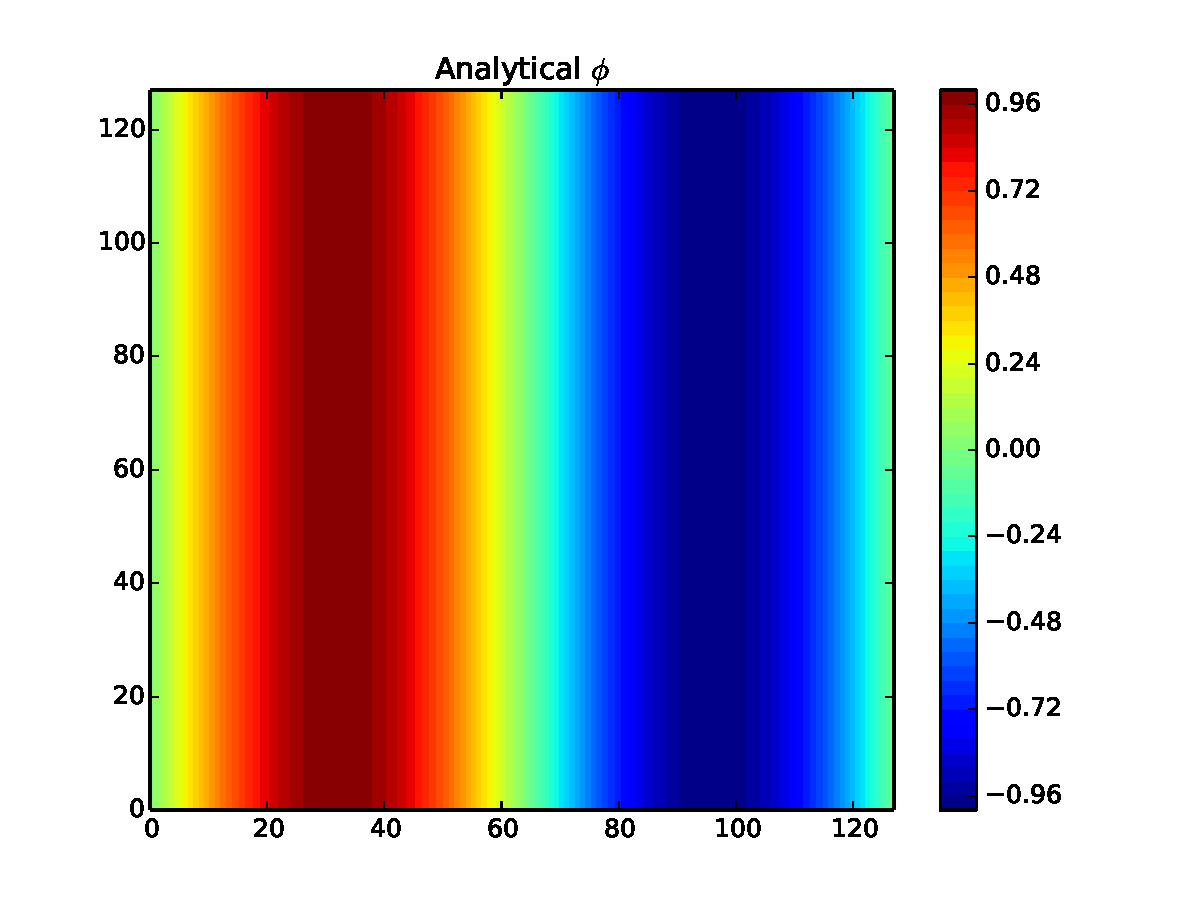
\includegraphics[width = 0.45\textwidth]{figures/verification/sinusoidal/analytical.pdf}
		% 	\end{subfigure}
		% 		\begin{subfigure}
		% 	% 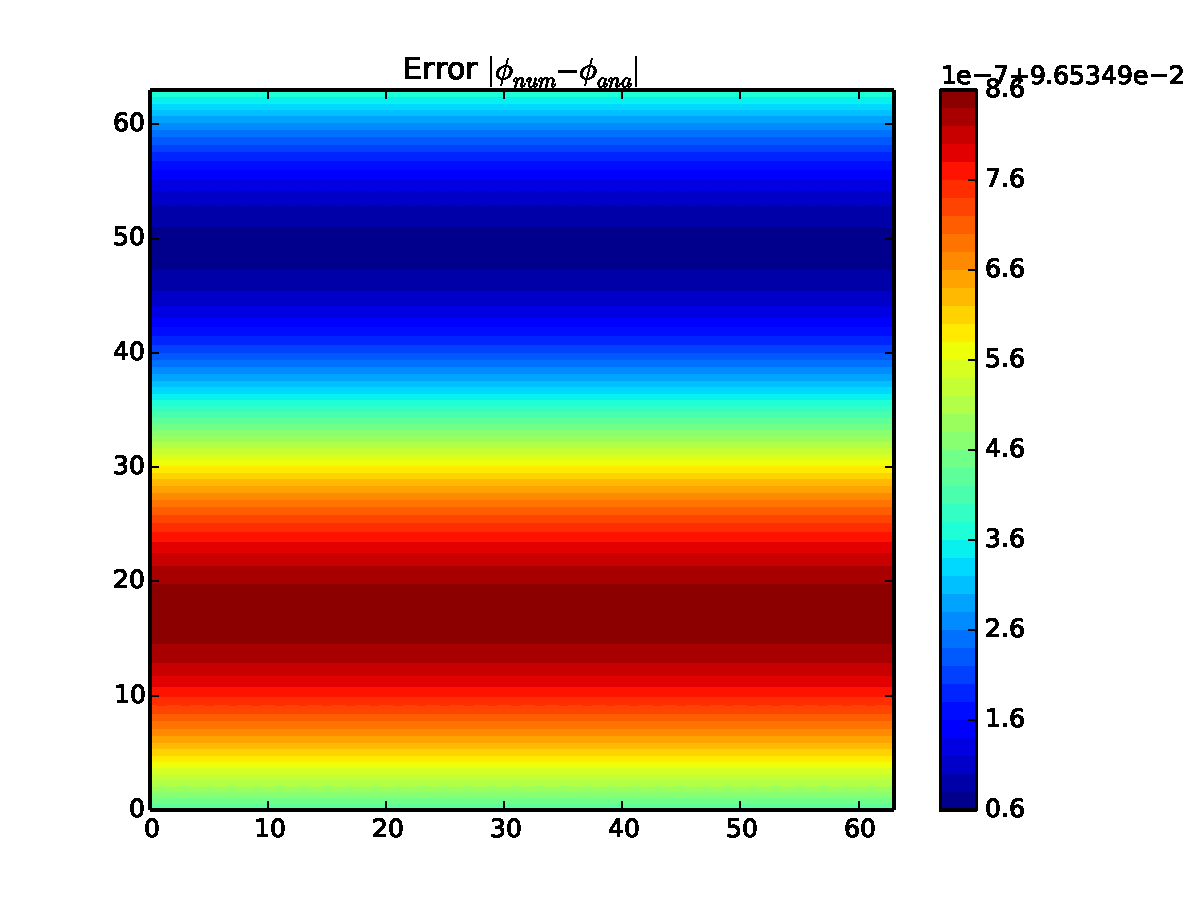
\includegraphics[width = 0.45\textwidth]{figures/verification/sinusoidal/error.pdf}
		% \end{subfigure}
		% \end{figure}
		%



		\subsection{Convergence of Residual}

		\subsection{Different Domain divisions}

% \section{Particle-in-Cell}
%
% 	\subsection{Plasma Oscillations}
%
% \textbf{NB! See if something below is salvageable}
%
%
% The multigrid method has several different steps in the algorithm, as a developmental
% help and to ensure that the program works correctly during as many different conditions
% as possible we want to test the whole code, as well as the constituent parts where possible.
% The method is quite modular and several parts of it can be tested alone.
% The GS-RB, used for smoothing, can be independently tested, since on it's own it converges to a solution,
% just at a higher computational cost than the multigrid method. To test it we will
% use an initial density field with a length between the grid steps that results in
% an exact answer. The restriction and prolongation operators can also tested to a
% degree by checking that they preserve a constant grid through several grid level changes.
%
%
% The multigrid method has several different steps in the algorithm, as a developmental
% help and to ensure that the program works correctly during as many different conditions
% as possible we want to test the whole code, as well as the constituent parts where possible.
% The method is quite modular and several parts of it can be tested alone.
% The GS-RB, used for smoothing, can be independently tested, since on it's own it converges to a solution,
% just at a higher computational cost than the multigrid method. To test it we will
% use an initial density field with a length between the grid steps that results in
% an exact answer. The restriction and prolongation operators can also tested to a
% degree by checking that they preserve a constant grid through several grid level changes.
%
% \subsection{The Multigrid method}
% 	We use both of the aforemented tests to check that the whole multigrid method
% 	works as intended. Since a constant source term will give a trivial solution of
% 	the potential, \(\phi(x,y,z) = \va{0}\), we use that as a test. In addition we
% 	also test that it converges on a sinusoidal source term as we did the smoother.
%
%
% \subsection{Smoothers}
%
% 	The iterative method GS-RB used for the pre- and postsmoothing of the grid in
% 	our implementation of the multigrid method is also a direct solver.
% 	So we can test it, or most other smoothers, by testing them on a small system
% 	where the problem has an analytical solution. Then we can let them run for a
% 	while and ensure that they are converging towards the solution. If we let
% 	the source term be sinusoidal in one direction, and constant in the other
% 	directions it has an easy solution given below
%
% 	\begin{align}
% 		\nabla^2 \phi(x,y,z) &= \sin(x)
% 	\end{align}
%
% 	This has a solution when \(\phi(x,y,z) = -\sin(x)\) and we can test that the
% 	solver converges to the solution. If we let the source term be constant in the
% 	x direction and instead vary in the other directions we can get verify that the
% 	solver works in all three directions independently.
